\section{Introduction}
\label{sec:introduction-rep}

Another application of the STAMM model is to reprogramming of somatic cell to a pluripotent state as investigated in \cite{Armond:2013}. In the experimental setup a mouse embryonic fibroblasts (MEFs) is used and transformed to a state of pluripotency \citep{Takahashi:2006hi,Jaenisch:2008cz} {\color{red} [15]}. More specifically we apply the model to the genome-wide microarray gene expression time-course data obtained by \cite{SamavarchiTehrani:2010cp}. It is a system that has been extensively studied in recent years and it is suggested that the reprogramming process is inherently stochastic \citep{Hanna:2009ix}. Progress has also been made on a single-cell investigations of the biological system \citep{Buganim:2012hp} {\color{red} ([20, 21, 22])}. Question still remain on genome-wide level including the number of intermediate state between the initial MEF state and the final pluripotent state. 

In this Chapter we start by briefly outlining results obtained \cite{Armond:2013} when applying STAMM to a microarray data set in Section \ref{sec:iPsc-results}. Then (in Section \ref{sec:test-single-cell}) we discuss the main contribution in detail which is a comparative study of parameters obtained from STAMM and single cell experiments performed by \cite{Buganim:2012hp}. The single cell data was obtained by a new kind of experimental technique called a Fluidigm assay. This also illustrates an example of a possible next step in investigating a biological system once parameters from STAMM have been obtained. 

\section{Results from model application}
\label{sec:iPsc-results}

\subsection{Differences in estimation}
\label{sec:diff-estim}

The initial step before we can make a comparison to single cell results is to apply STAMM to the microarray time-course; obtaining single cell level parameters and the number of states $K$. In  \cite{Armond:2013} there are differences in the estimation pipeline compared to the one outlined in Section \ref{sec:estim-pipe}.

The main idea of a two-step estimation process is shared. The first difference is that the optimal number of clusters is chosen when increasing the number of clusters does not significantly improve the k-means objective function. The penalty for estimation used to regularise estimation in eqn. (\ref{eq:leastSqrs.indep}) is set to a small positive number (in this application set to $ \lambda = 0.1 $). Estimation of transition rates $\lbrace \mathbf{w} \rbrace $ is performed on genes closest to cluster centroids instead of the cluster centroids themselves; then transition rates are fixed and estimation of expression signatures $\beta_{kj}$ is performed in the same way. Finally estimation of the number of states $\hat{K}$ is performed in two ways. The heuristic approach is to looks at two quantities the model fit, i.e. the residual sum-of-squares (RSS), and the distinctness for individual state signatures quantified by the condition number $C = \max(s_i) / min(s_i)$; where $s_i$ are the singular values of a matrix made up of the expression signatures. The other approach for finding an optimum number of states is employed for genes closest to centroids using a Bayesian model selection approach. Let $\mathbf{y} = \lbrace y_j \rbrace$ denote observed data and $M_k$ the model with $k$ states. The posterior probability is $P(M_n | \mathbf{y}) \propto p(\mathbf{y}|M_k) $ with a flat prior distribution over models. The marginal likelihood $p(\mathbf{y} | M_k)$ accounts for the fit-to-data and model complexity. Writing all model parameters as $\theta = (\beta_{kj}, \lbrace \mathbf{w} \rbrace, \lbrace \sigma_j \rbrace) $ the marginal likelihood is:

\begin{equation}
  \label{eq:marginal-model}
  p(\mathbf{y} | M_k) = \int p(\mathbf(y) | \theta, M_k)\, p(\theta | M_k) d\theta.
\end{equation}

We compute the marginal likelihood of the model eqn. (\ref{eq:marginal-model}) using annealed importance sampling (AIS) \citep{Neal:2001ed}, a MCMC method, to compute the marginal likelihood. Hyperparameters for this model are set by hand to reasonable values, see Supplement of \cite{Armond:2013} for details. The normalised score is the required posterior probability over the number of states. 

\subsection{Estimation results}
\label{sec:estimation-results}

The primary data used in \cite{Armond:2013} is obtained by reprogramming of a secondary mouse embryonic fibroblast (MEF) where Oct4, Sox2, Klf4, and cMyc are inducibly expressed in the system for 30 days \citep{SamavarchiTehrani:2010cp}. Microarray measurements were made at $t = \lbrace 0, 2, 5, 8, 11, 16, 21, 30 \rbrace$ days after induction of expression factors. The microarray data is standardised per gene such that $y_j(t) = \left(z_j(t) - \mu_j \right) / \sigma_j$, where $z_j(t)$ is original $\log_2$ transformed data, $\mu_j$ is the mean and $\sigma_j$ is the standard deviation of the time course data for gene $j$. A total of $4383$ genes are retained out of the whole gene list. Genes are removed if they are expressed at very low levels and therefore would be dominated by noise. 

\begin{figure}[!t]
  \centering
  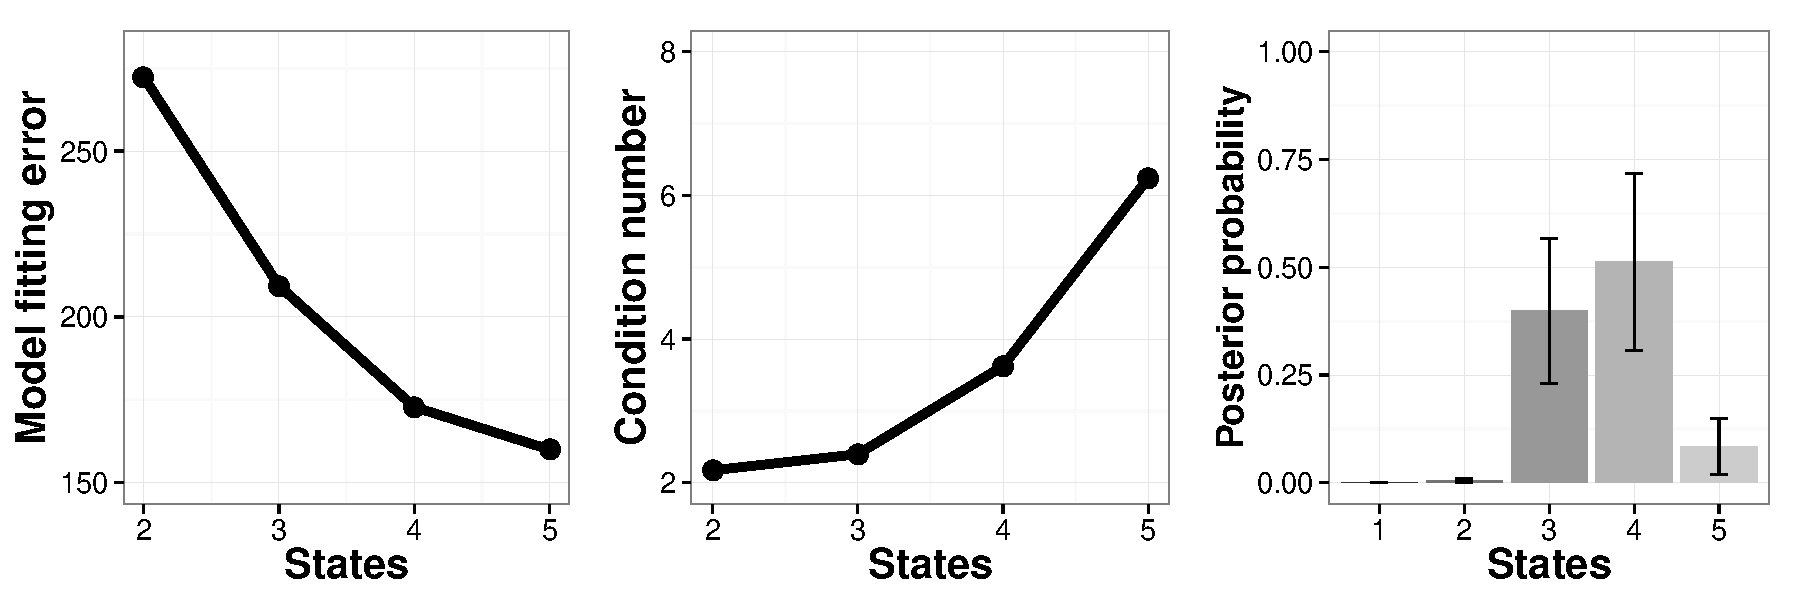
\includegraphics[width=1\textwidth]{pics/rss_rcond_bay1.pdf}
  \caption{Application of STAMM to a microarray time-course (a) Plot of the model fit residual sum of squares (RSS). (b) Plot of the condition number for estimated expression signatures quantifying linear dependence between states. A larger number corresponds to more dependence. (c) Posterior probabilities obtained from Bayesian model selection (see Section \ref{sec:diff-estim} for details).}
  \label{fig:model-fit-repro}
\end{figure}

The number of clusters chosen for this data set of $8$ time points is $\hat{m} = 7$. As mentioned above the penalty used in this application is $\lambda = 0.1$. With these parameters set the transition rates are estimated from cluster representative genes. Once transition rates are estimated the expression signatures for the remaining genes are estimated. The analysis is carried out for $K = \lbrace 2 \ldots 5 \rbrace $ and results for model selection are summarised in Figure \ref{fig:model-fit-repro}. Unsurprisingly the RSS keeps decreasing for increasing $K$ (Figure \ref{fig:repro-rss}) since numbers of model parameters increase. To determine number of states heuristically we compare these results with the condition number (Figure \ref{fig:repro-cond}). We find that the difference in condition number from $K=4$ to $K=5$ is larger than the preceding changes. This suggests that decrease in RSS from $4$ to $5$ states is mostly due to overfitting and the additional state is not distinct. The posterior probabilities form Bayesian model selection for $7$  genes closest to the centroid (see above for details), are shown in Figure \ref{fig:repro-bay}. Combined these results indicate that a $\hat{K} = 4$ since it strikes a good balance between model fit and distinct expression signatures for states as well as having the highest posterior probability. 

\begin{figure}
  \centering
  \subfigure[RSS]{
    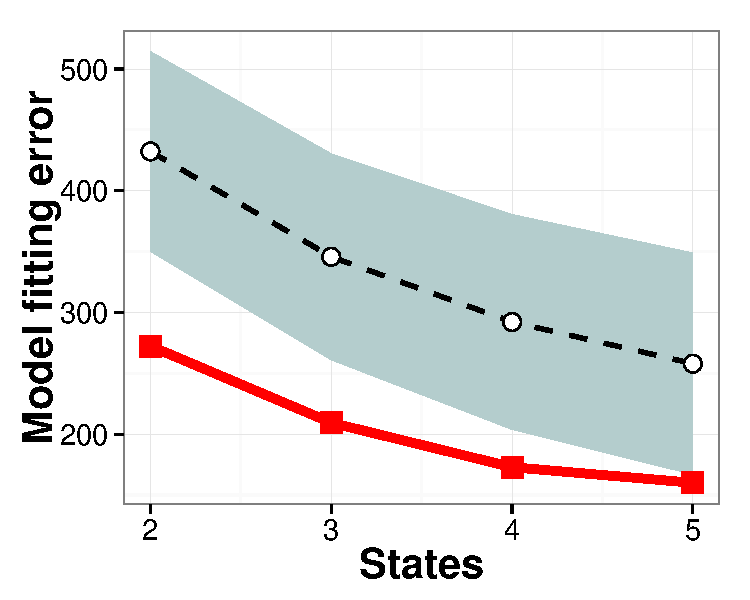
\includegraphics[width=0.3\textwidth]{pics/supp_fig_randomised3.pdf}
    \label{fig:repro-rss}
  }
  \subfigure[Condition number]{
    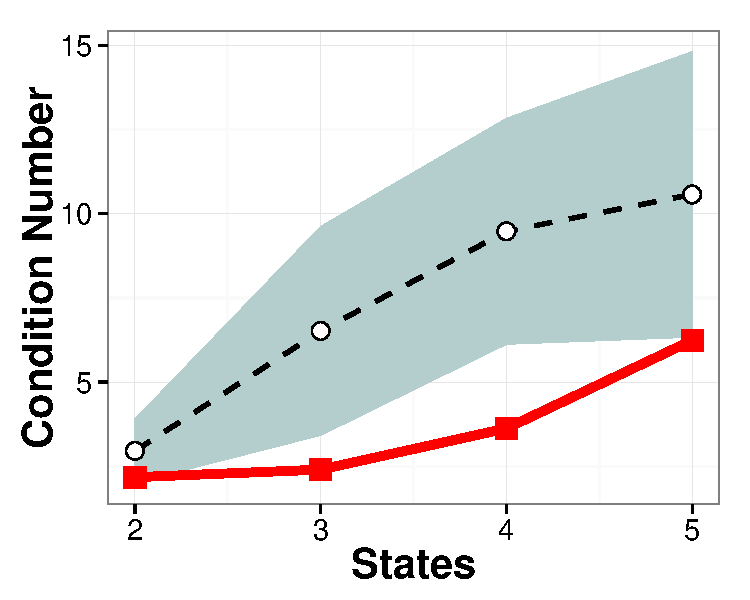
\includegraphics[width=0.3\textwidth]{pics/supp_fig_randomised4.pdf}
    \label{fig:repro-cond}
  }
  \subfigure[Bayesian model selection]{
    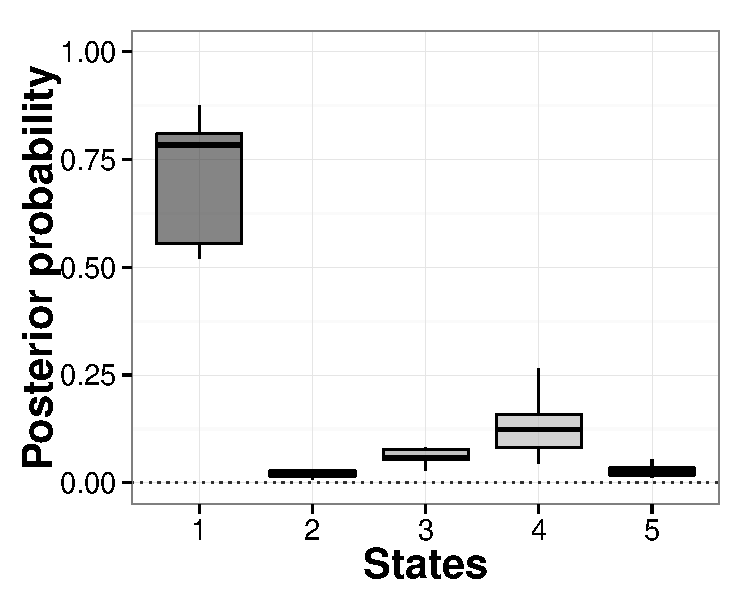
\includegraphics[width=0.3\textwidth]{pics/supp_fig_randomised1.pdf}
    \label{fig:repro-bay}
  }
  \caption{{\color{red} Random permutation of time points. a, model fitting error, b, reciprocal condition number and c, Bayesian posterior probability as a func- tion of number of states. We generated a set of randomized data by random reordering of time indices and the model was re-fit for each of the permuted data. Curves (a,b) and box plots (c) shown are over ten samples; in (a,b) dotted lines indicate means and the shaded area standard deviations, whilst the cor- responding result for the correct time ordering is shown in red. Both model fit and distinctness of state signatures are systematically worse under permutation of time indices. Bayesian model selection applied to the randomly permuted data show no evidence of intermediate states (c), in contrast with the original data (Fig. 2c, Main Text). [Dataset from Samavarchi-Tehrani et al. [1]; see SI Text for details.]}}
\label{fig:permutation-repro}
\end{figure}

\section{Testing against single cell data}
\label{sec:test-single-cell}

\subsection{Single cell experiment}
\label{sec:single-cell-exper}

Results in Section \ref{sec:estimation-results} are obtained analysing homogenate time-course data; but the transformation process is on a single cell level therefore it is of interest to study behaviour on a single cell level. Comparing results from STAMM to single cell observations also indicates how well the underlying single cell process is modelled. For this purpose we investigate the mRNA single-cell expression performed by \cite{Buganim:2012hp}. They also investigate a secondary MEF system reprogrammed by transduction of Oct4, Sox2, Klf4, and cMyc; obtaining data with the Fluidigm assay, resulting in $96$ single-cell measurements with gene expression from $48$ genes. Observations are made in populations, starting with MEFs, over cells at $2 - 6$ days during reprogramming, to the final reprogrammed cells.

\subsection{Comparing results}
\label{sec:comparing-results}

The single-cell measurements \citep{Buganim:2012hp} allow for analysis that has not been possible for population average data. Although important questions about the transformation process such as the number of states and transition rates still remain difficult to track down; this is due to the fact that each time a single-cell measurement is made the cell has to be destroyed and additional work is necessary to determine distinctive marker for known states for purification. 

Given available data we can address interesting question on expression patterns; since we assume that cells belonging to the same states would have a comparable expression patterns across observed genes. This is especially the case since measured genes are deemed important for reprogramming. To this end we cluster the data for all cells in a $48$ dimensional gene expression space. To perform the clustering we use a widely available clustering tool in R mclust; it employs a variety of multi-variate clustering methods and scores them using the Bayesian Information Criterion (BIC). The best performing method is shown in Figure \ref{fig:buganim-mclust}. We find that optimal number of clusters is $3$ since the BIC score starts decreasing for larger cluster sizes. 

\begin{figure}[!t]
  \centering
  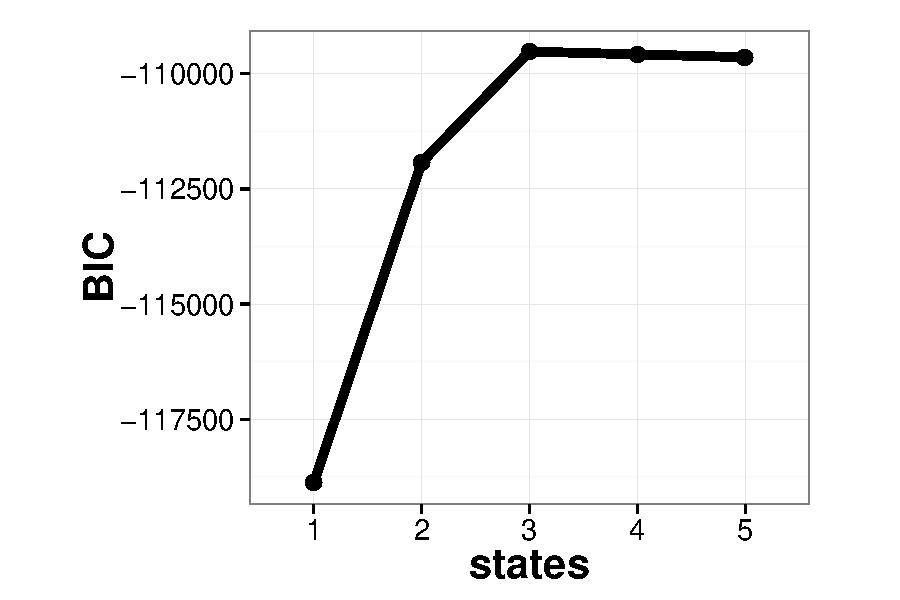
\includegraphics[width=0.6\textwidth]{pics/yossi_mclust.pdf}
  \caption{Single cell expression levels in different experimental settings from \cite{Buganim:2012hp} are clustering using a standard clustering procedure in R called mclust. We use the Baysian Information Criterion (BIC) to score different cluster sizes. We find the optimal number of clusters to be $3$ since the BIC score decreases for larger cluster sizes.}
  \label{fig:buganim-mclust}
\end{figure}

Next we try to determine if state specific expression signatures estimated from microarray data can be compared with this new single-cell data. Disregarding conditions for each cells measurement we assign each of the single-cell measurements to the each of the states in the $K=4$ model. We compute the euclidean distance between gene expression on a single-cell level and estimated gene expression signatures and assign each cell to a specific state. The heatmap in Figure \ref{fig:buganim-heat} shows fractions of cells that are assigned to each state. All MEF conditions have a peak at $K=1$. Measurements obtained between $t=2$ and $t=44$ days are spread over state $K=1$ and $K=3$ with very few cells also in the second state. No cells from each of these measurement are close the final state. Measurements for dox-independent and iPS cells occupy only the final two states. These results clearly show a transformation starting with MEF state and undergoing changes across intermediate states before reaching the final reprogrammed state. Of course this is a very small study and a study made on a slightly different system under different conditions therefore even the approximate similarities we find to our estimated parameters are promising. 

\begin{figure}
  \centering
  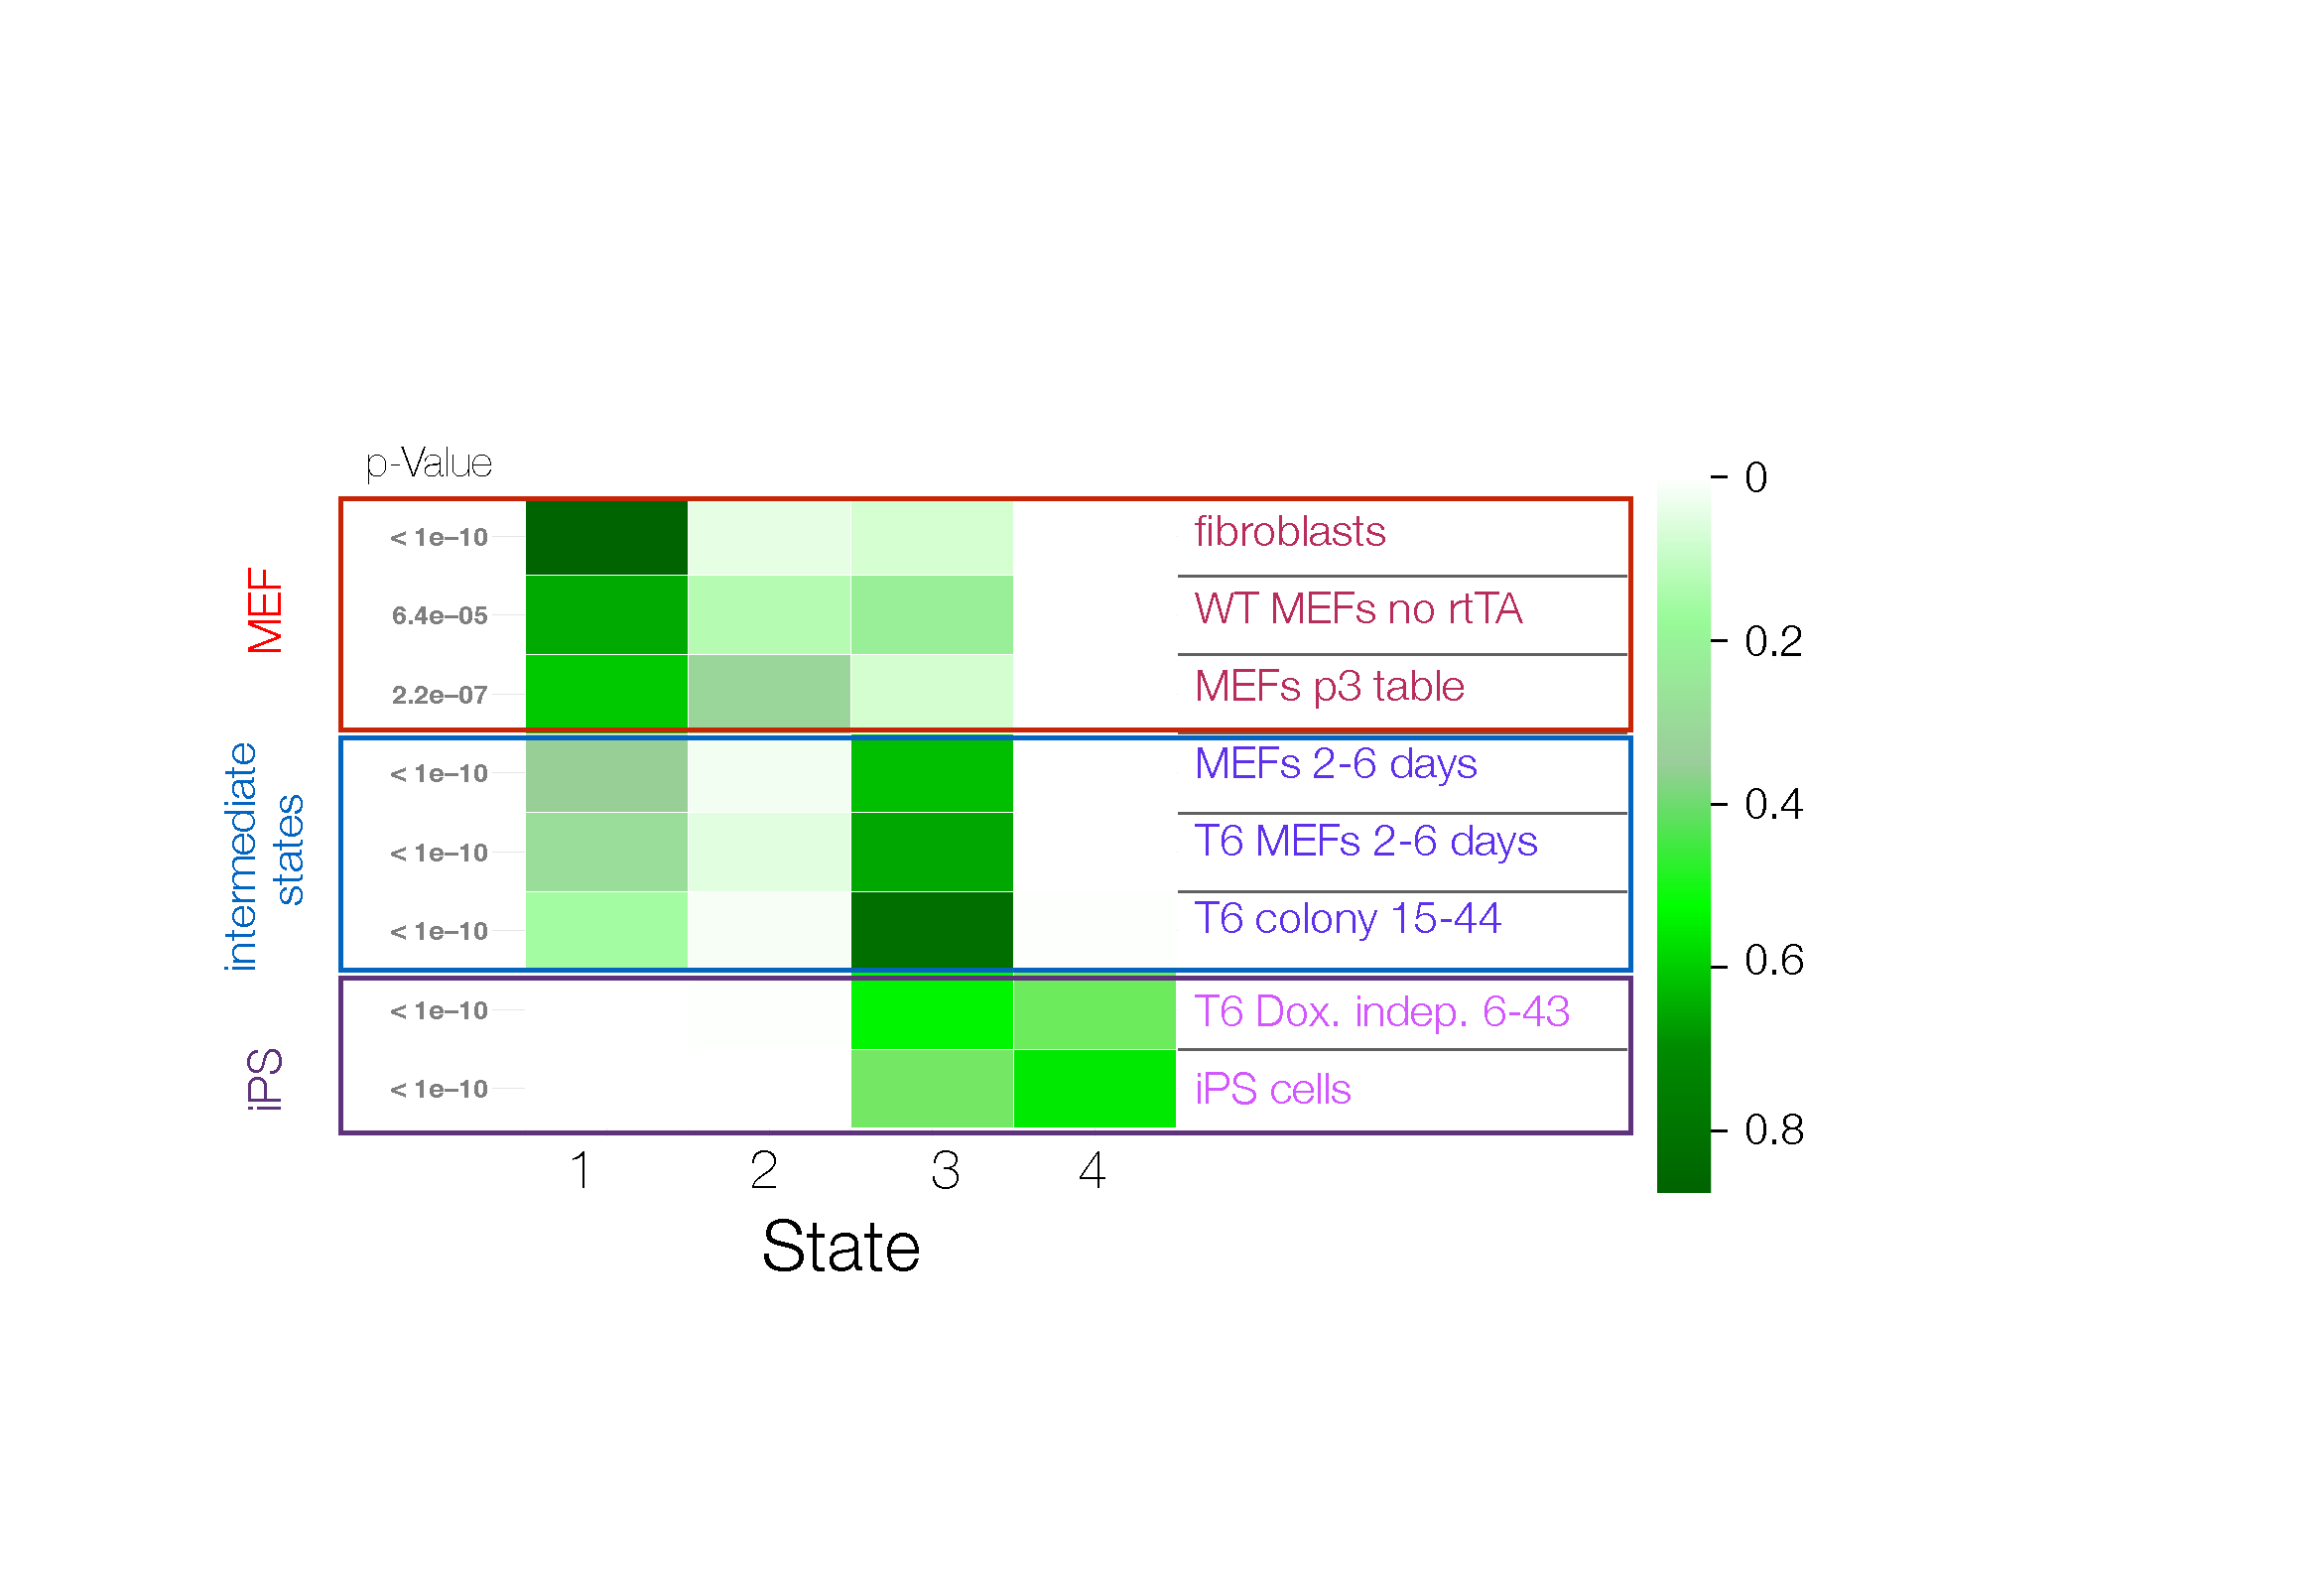
\includegraphics[width=0.9\textwidth]{pics/Heat_single_cells.pdf}
  \caption{Estimated gene expression signatures using STAMM are compared with single-cell measurements performed by \cite{Buganim:2012hp}. Each single-cells is assigned to a state by finding minimum euclidean distance. The heatmap summarises the fraction of cells from each experimental condition assigned to specific states. Different conditions show a clear preference for specific states. The prediction of our model are in line with this observation where initial MEF states undergo a transformation via intermediate states to a final reprogrammed state. As an example all MEF populations (top three entries) have a significantly higher fraction of cells in $K=1$. Cells measured between $t=2$ and $t=44$ days have cells in the spread across the first and third state with very few cells occupying the second state. None of these cells are close to the final state. The two measurements which are reprogrammed cells (iPS cells and Dox. indep.) show similarities to $K=3$ and $K=4$, but none of these cells are close to the first two states.
}
  \label{fig:buganim-heat}
\end{figure}


%%% Local Variables:
%%% TeX-master: "warwickthesis"
%%% End:
